\documentclass{article}
\usepackage[margin=0.5in]{geometry}
\usepackage{graphicx}

\title{Rutgers CS 440 Homework 1}
\author{Fulton Wilcox III, Dan Teytel, Long Tran}
\date{February 17 2023}

\begin{document}

\maketitle

    \begin{enumerate}
        \item[1.] \textbf{Understanding the Methods}
        \begin{enumerate}

            \begin{figure}[h!]
			\IfFileExists{diagram.png}{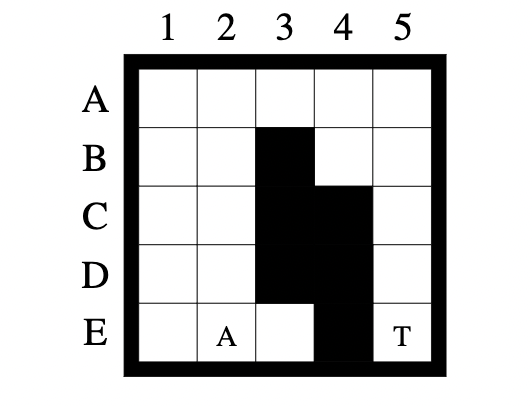
\includegraphics[width=0.2\textwidth]{diagram.png}}{No Figure Yet}
		\end{figure}
            
            \item[a.] In this example, the first move from A to the target will be to the right rather than up because the heuristic, which is the Manhattan distance from the current spot to the target, is 2 for the spot E3, while the heuristic for spot D2 is 4.  The step cost is 1 for both since this is the first step, so f(E3) $<$ F(D2).

            \item[b.] Using A* search, the agent either reaches the target or discovers that it is impossible to reach the target.
            To argue this, consider an agent and a target at any arbitrary spots on an arbitrarily generated maze.  An agent can expand its current node in any direction if that particular cell is unblocked and then move to the cell that has the lowest f(n).  Assuming the target is unreachable, as long as there is an unblocked cell adjacent to an expanded cell, A* will not terminate.  Therefore, in the worst case, A* will terminate only when there are no longer any adjacent un-expanded cells.  In the case when there is a path to the target, A* will terminate when every other path has greater cost than the cost to the target.
        \end{enumerate}
    \end{enumerate}


\end{document}
